\chapter{Validation}\label{ch:validation}

In this section we will talk about the \textbf{testing part} and the validation 
of the project. 
In particular our purpose was to show that the \textbf{system satisfy the requirements} 
listed in ~\ref{ch:analysis}. \\

\noindent
Validation is a crucial aspect for this project because debugging in a distributed context 
is really hard moreover erlang increases the difficulty because it doesn't provide 
great tools for real time debugging.


\section{Web service validation}

As stated in the previous chapter~\ref{ch:implementation} web service logic is enclosed in the services 
so testing this logic with a unit tests (for unit testing we use a tool provided by erlang called EUnit~\cite{22})
implies the validation of the entire web service.

Note that the database isn't persistent, every time that the service restarts it is cleaned, 
so there was no need to create any moq fixtures for the database in order preserving the data during a testing session.


\section{Car validation}

Car validation was really hard cause it can interacts with some other cars and also with the 
web service. 

Anyway we have noticed that the entire massage traffic of a car passes 
through its supervisor; so at first we create an alternative test supervisor that 
emulates some conditions and testing the car responses (in terms of car state).

This kind of test was very useful cause we were able to check 
the correct message flow and also the state transitions.

In other words we wanted to find out if the car, in a 
particular situation (defined by the environment), reacts to it sending and receiving 
the expected events; the car should also act as we wanted so that there is no accident, 
deadlock, starvation and so on.


\subsection{Functional requirements validation}

We were able to check if the system can:
\begin{itemize}
    \item \textbf{Coordinate the traffic}.
    \item \textbf{Avoid} any kind of \textbf{accident}.
    \item Avoid situation where more than $c$ cars, where $c$ is the bridge capacity, 
        cross the the bridge at the same time.
    \item Make cars cars interchange messages due to decide correctly who can cross, after reached an
    (\textbf{agreement}), the bridge.
    \item Detect \textbf{broken} cars and remove them calling a tow truck.
    \item generate new cars.
\end{itemize}


\section{Non functional requirements}

For the non functional requirements we tested that:
\begin{itemize}
    \item \textbf{Safety}: the system guarantees that the bridge can be crossed only by cars that 
        are moving in the same direction, but also that if a car broke, the others are able to detect that
        and so they stop before crashing into it. 
    \item \textbf{Strength}: the system is usable even if a car breaks down and needs to be removed.
    \item \textbf{Scalability}: incrementing number of cars, clients and web services, the system don't affect
    too much the whole system.
    \item \textbf{Starvation}: when a car requires to cross the bridge, the request will be satisfied 
    eventually. 
    \item \textbf{Fairness}: the crossing order is a \textbf{FIFO ordering}.
\end{itemize}

Anyway this kind of test wasn't able to cover any possible interaction and also 
any possible scenery cause even if the problem seems quite simple the distributed 
aspect implies asynchronicity and concurrency (two aspects that cannot be reproduced 
in a deterministic way as would be done in a unit test).

At a second time we decided to implement several key scenerys in order to see what will actually happen. 
In the following sections there are also some significant screenshot we took from the UI while running 
different scenerys. 

Scenerys are basically \textit{.json} files stored in the client assets which 
can instantiate any number and type of cars. 
The following are the property of each scenery:
\begin{itemize}
    \item[\fbox{scenery \textbf{1}} $\quad$] There are two cars, on the same side (left), 
    while there is no one on the other side. 
    The cars don't arrive at the same time but there is a delay of $2000$ ms between them. \\

    \begin{center}
        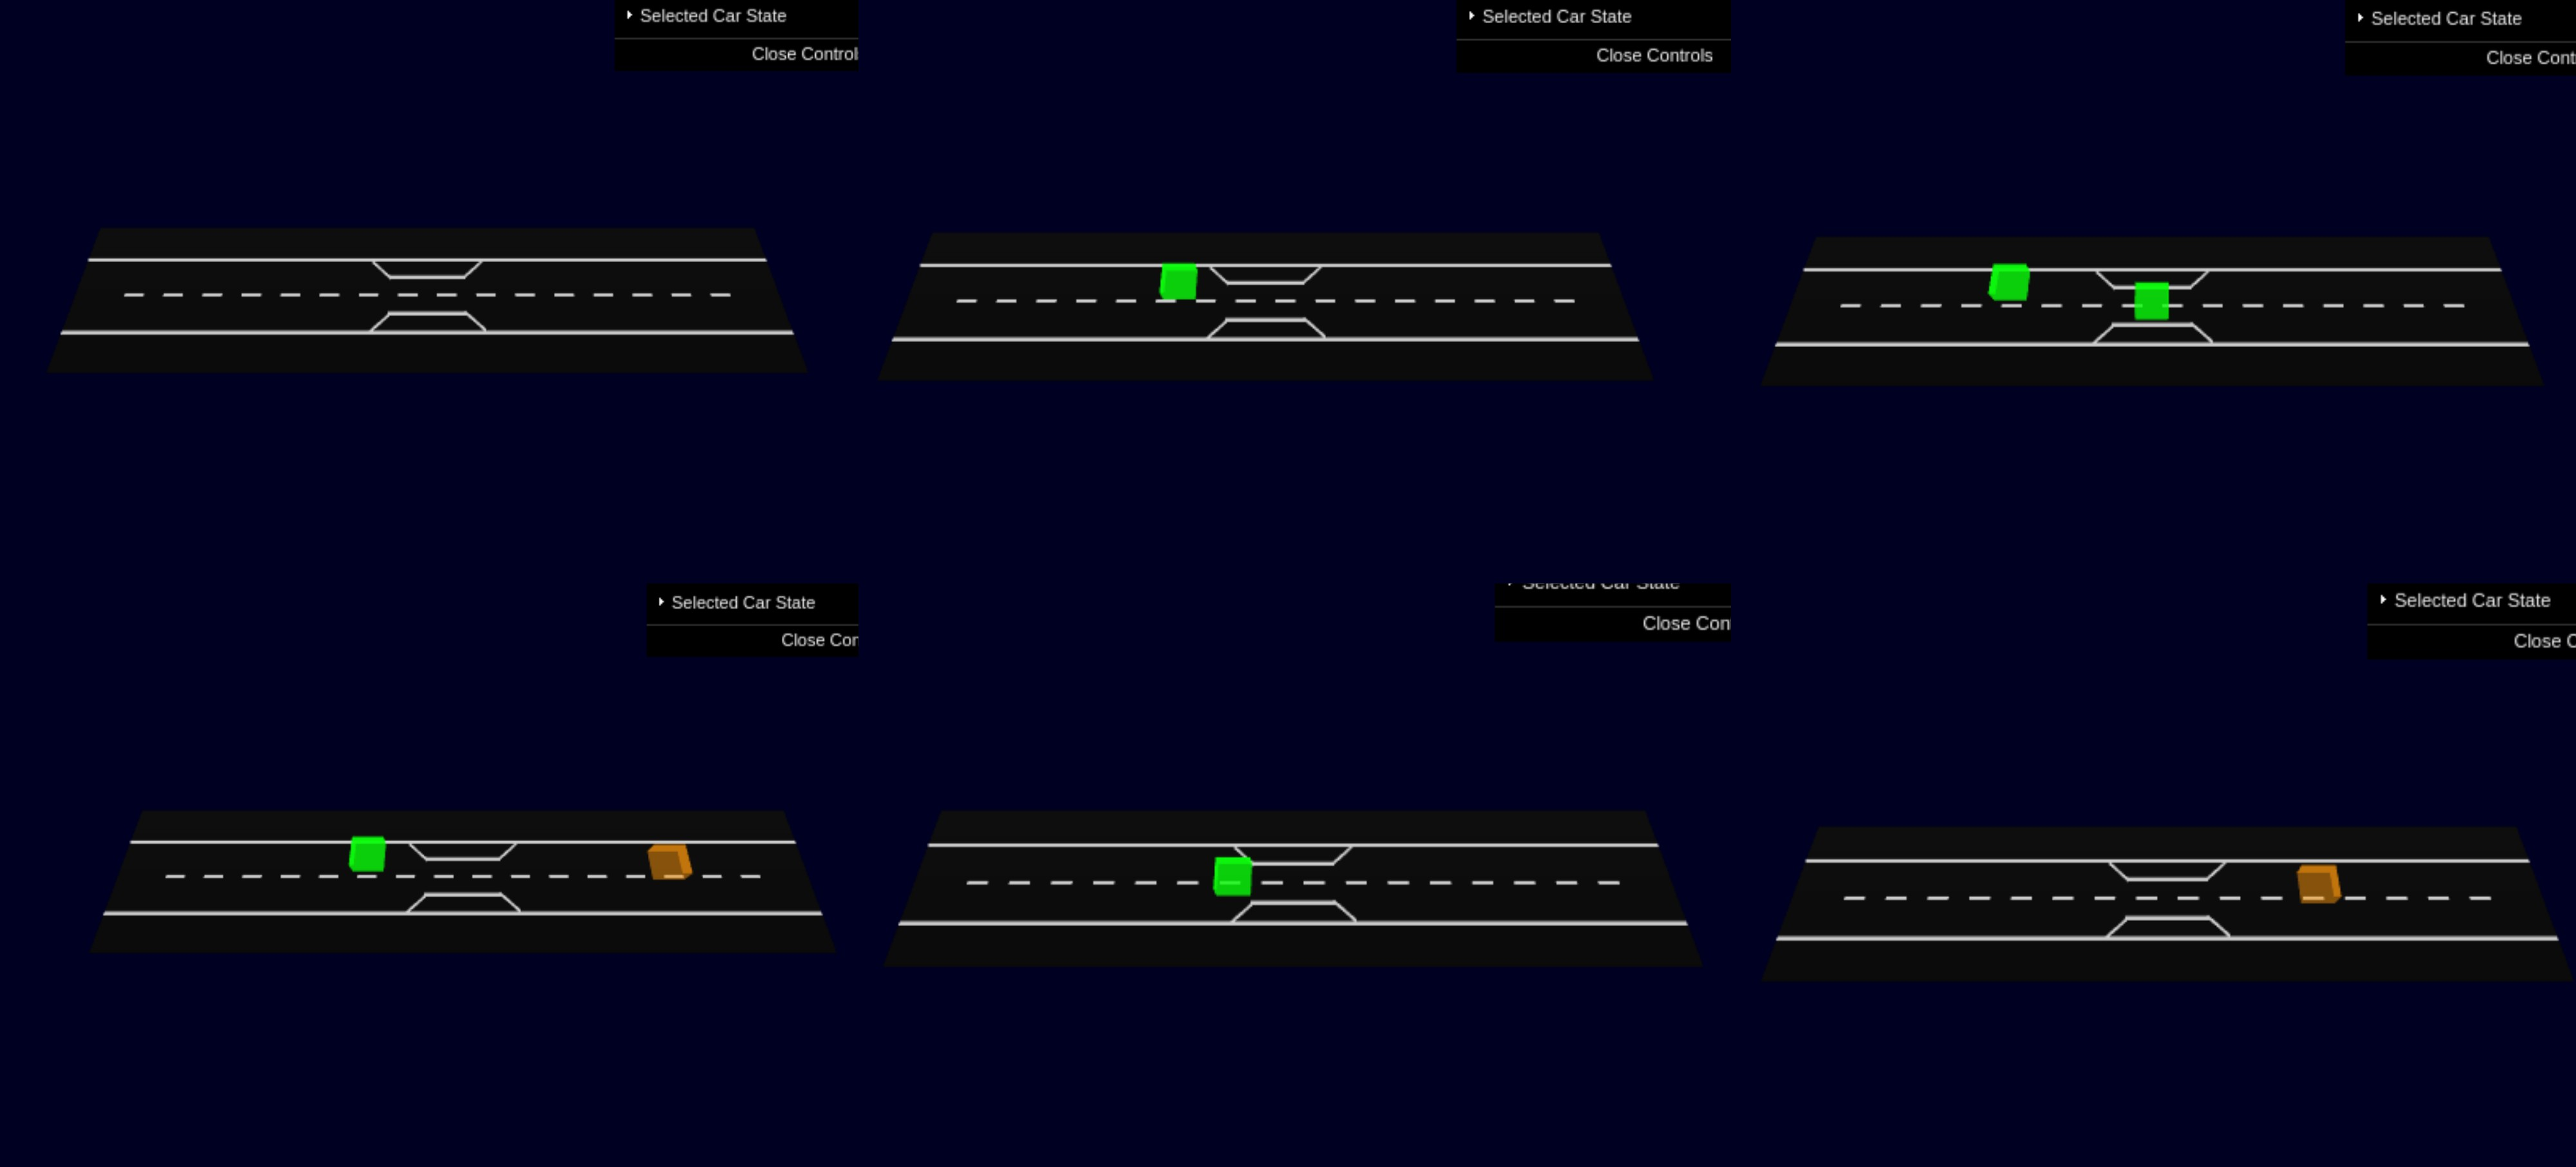
\includegraphics[scale=0.3, width=\linewidth]{assets/sc1.jpg}
        \captionof{figure}{scenery 1}
    \end{center}

    The correct behaviour should be that the first car that reach the bridge will cross it (the other 
    one will wait and then cross the bridge too) \\
    
    \item[\fbox{scenery \textbf{2}} $\quad$] There are five cars on the same side, all 
    created at the same time \\

    \begin{center}
        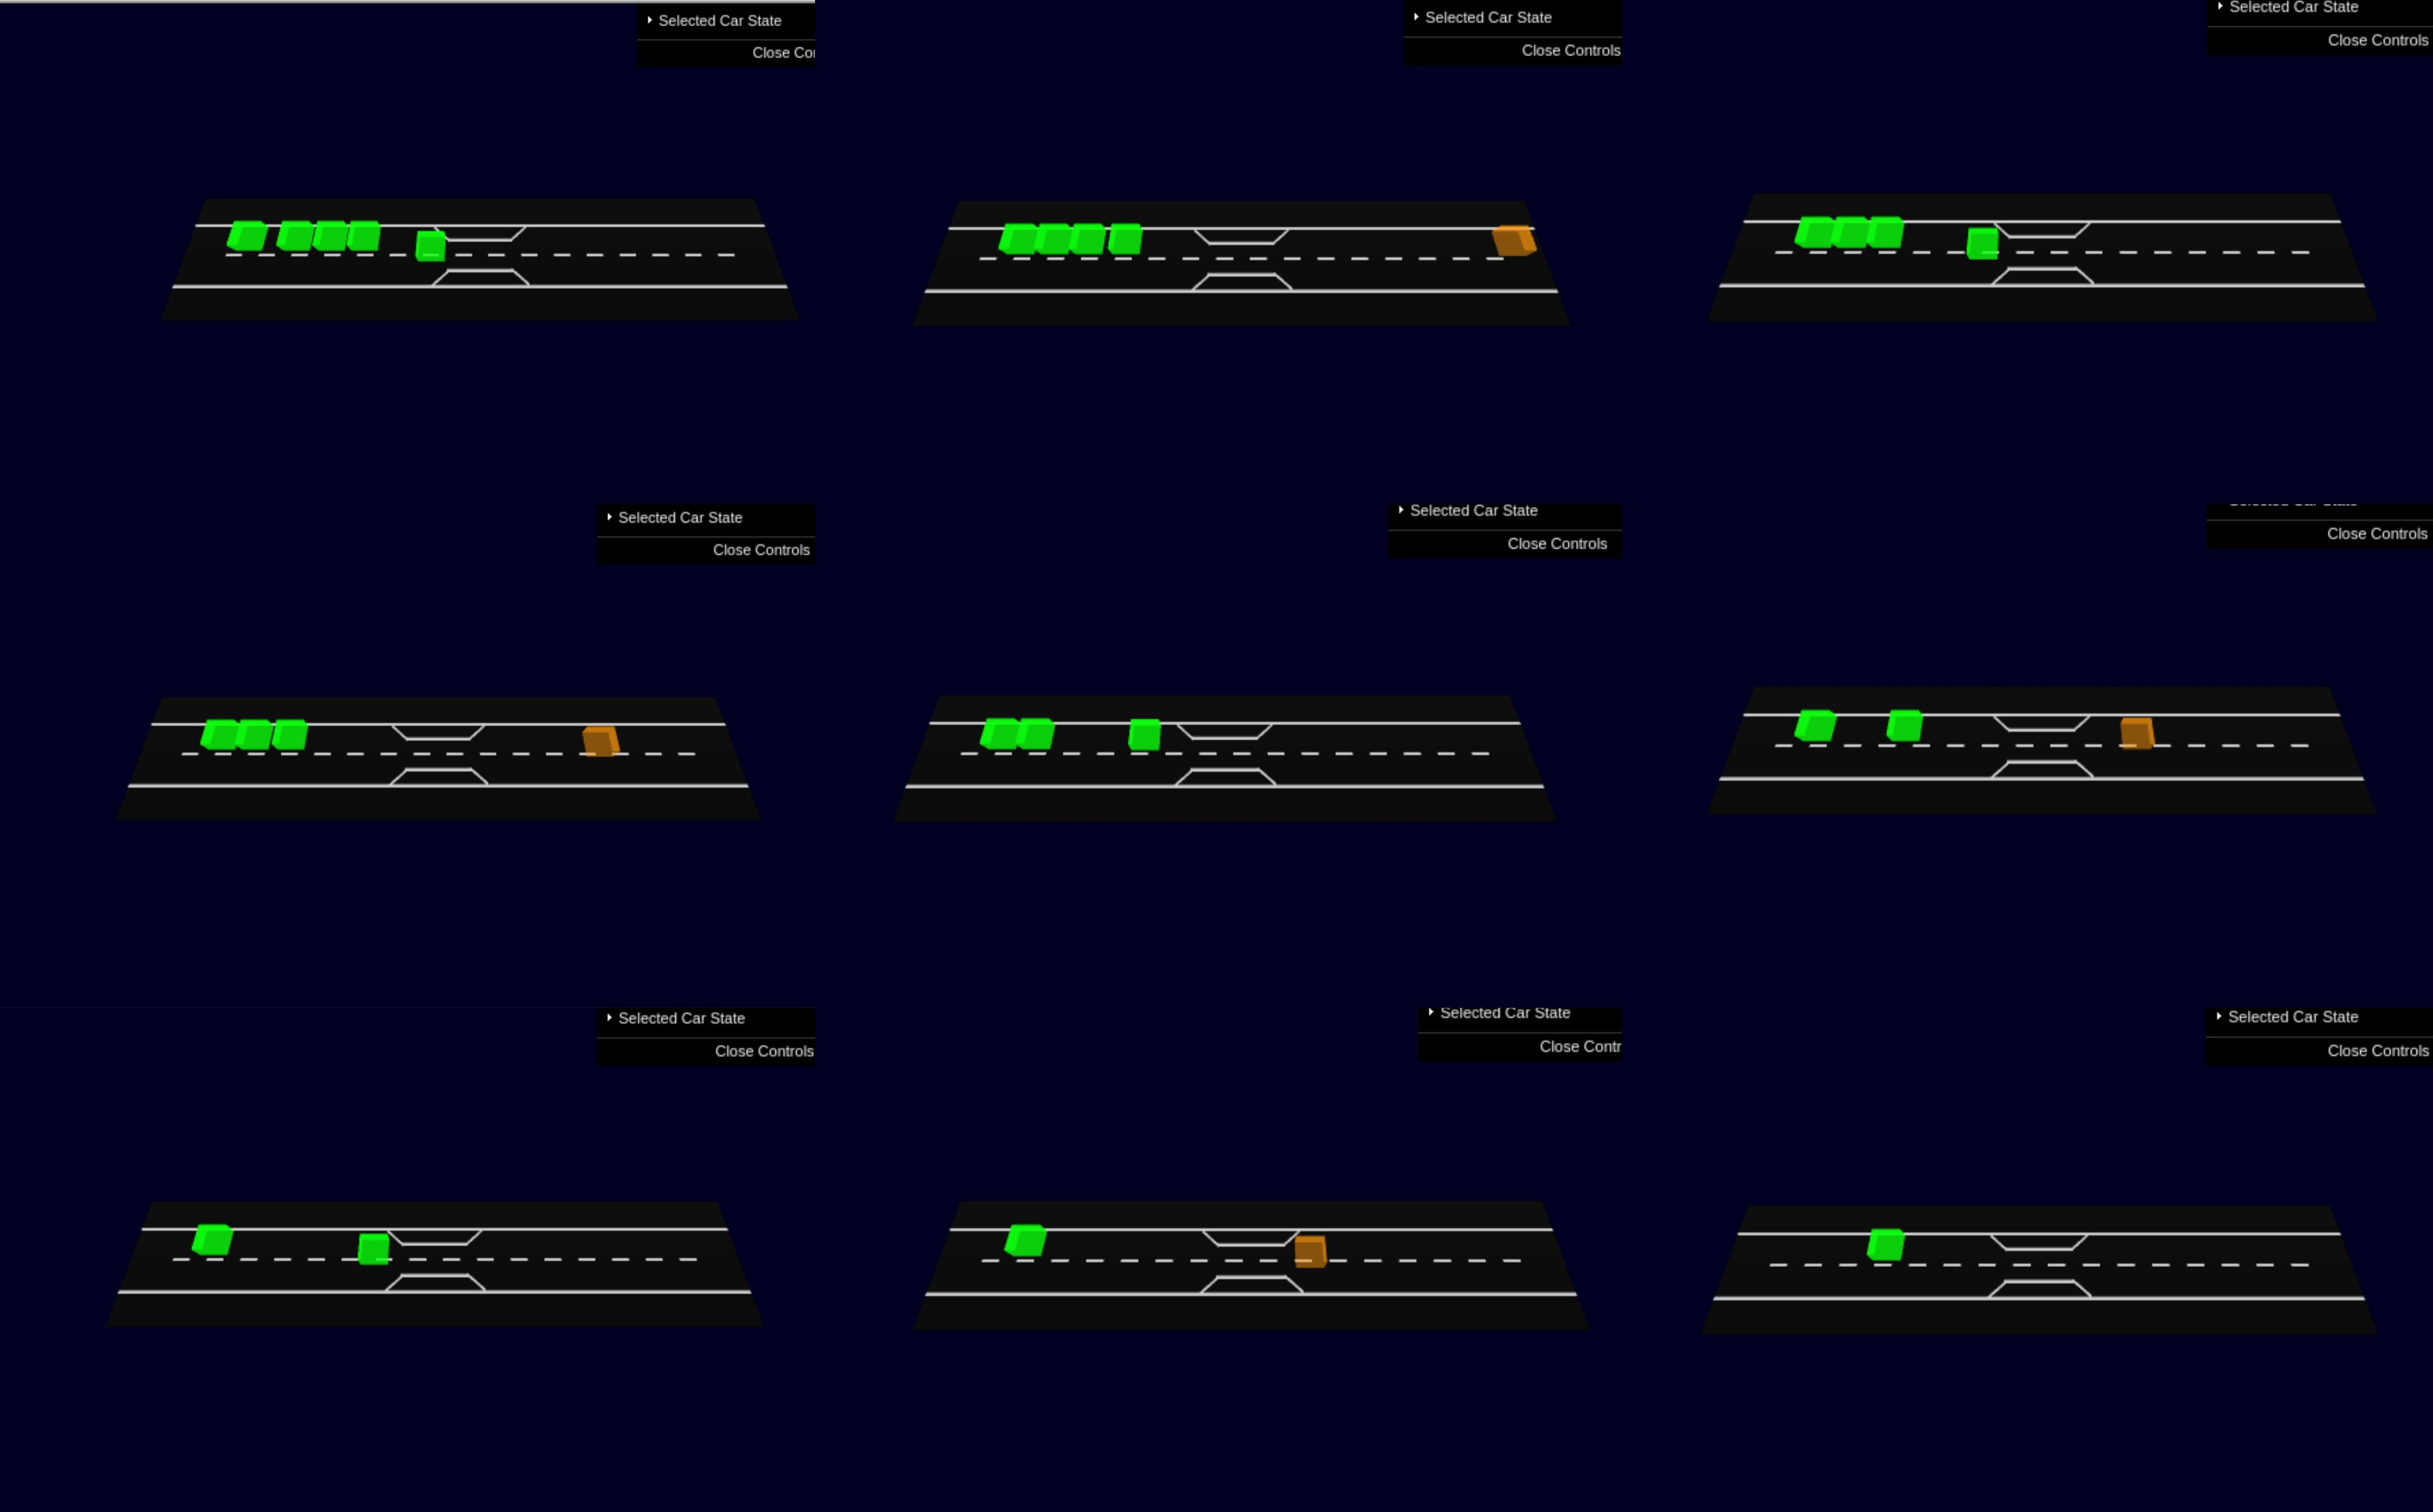
\includegraphics[scale=0.3, width=\linewidth]{assets/sc2.jpg}
        \captionof{figure}{scenery 2}
    \end{center}

    The correct behaviour should be that the cars are able to synchronize themselves 
    and then cross the bridge according to their $arrival\_time$ \\

    \item[\fbox{scenery \textbf{3}} $\quad$] There are four car on left side and one on the right side (there is no delay 
    between them).\\ 

    \begin{center}
        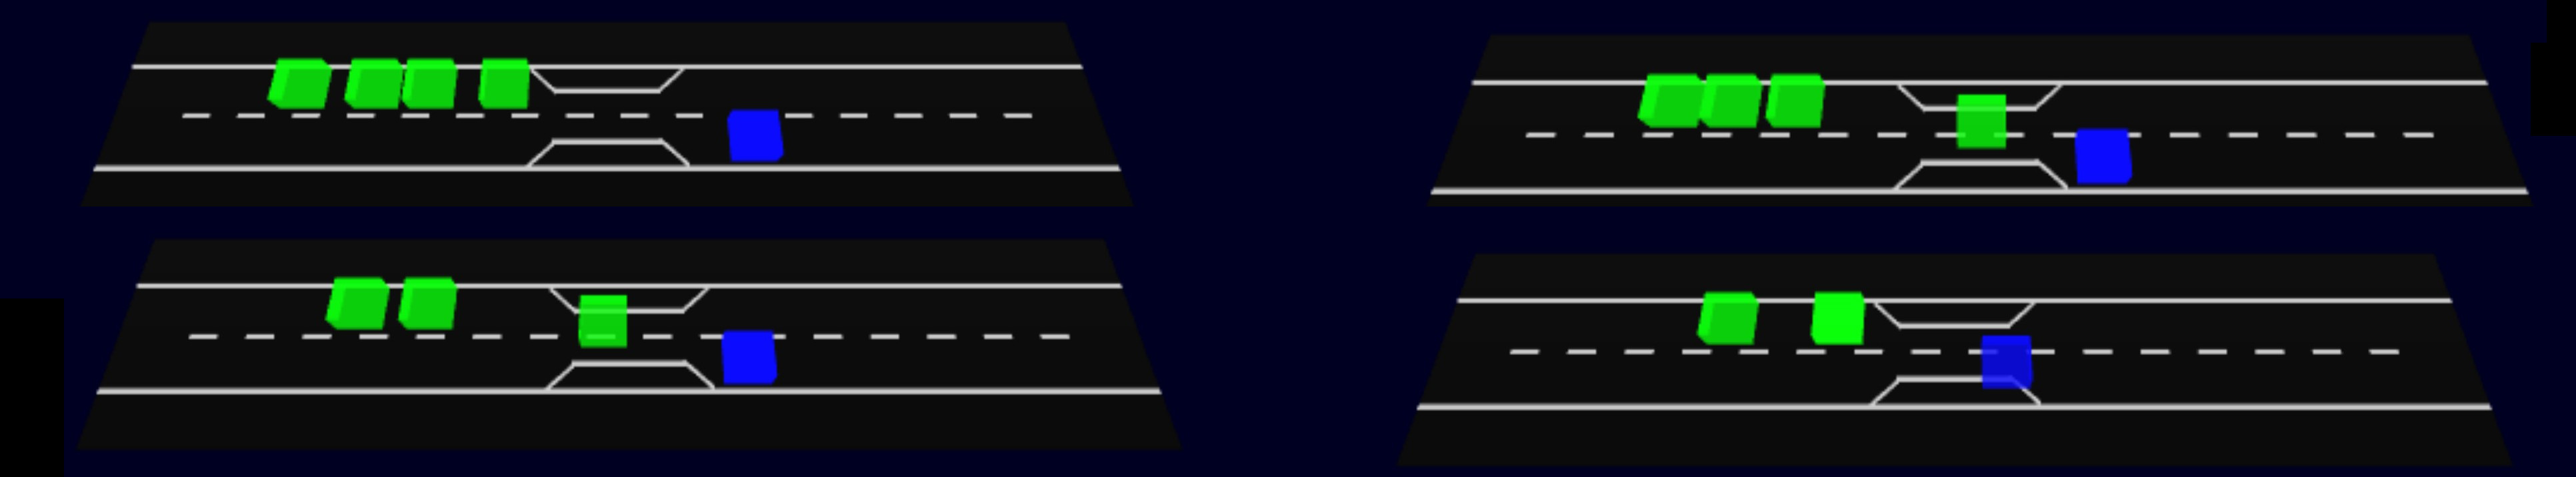
\includegraphics[scale=0.3, width=\linewidth]{assets/sc3.jpg}
        \captionof{figure}{scenery 3}
    \end{center}
    
    The correct behaviour should be that the cars will cross the bridge in the correct 
    order without crashing with the car on the other side (that will wait for its turn accordingly
    to its arrival time) \\

    \item[\fbox{scenery \textbf{4}} $\quad$] There are three cars, with no delay, that are on the same side but there is one that is going to
    have a system crash.\\ 

    \begin{center}
        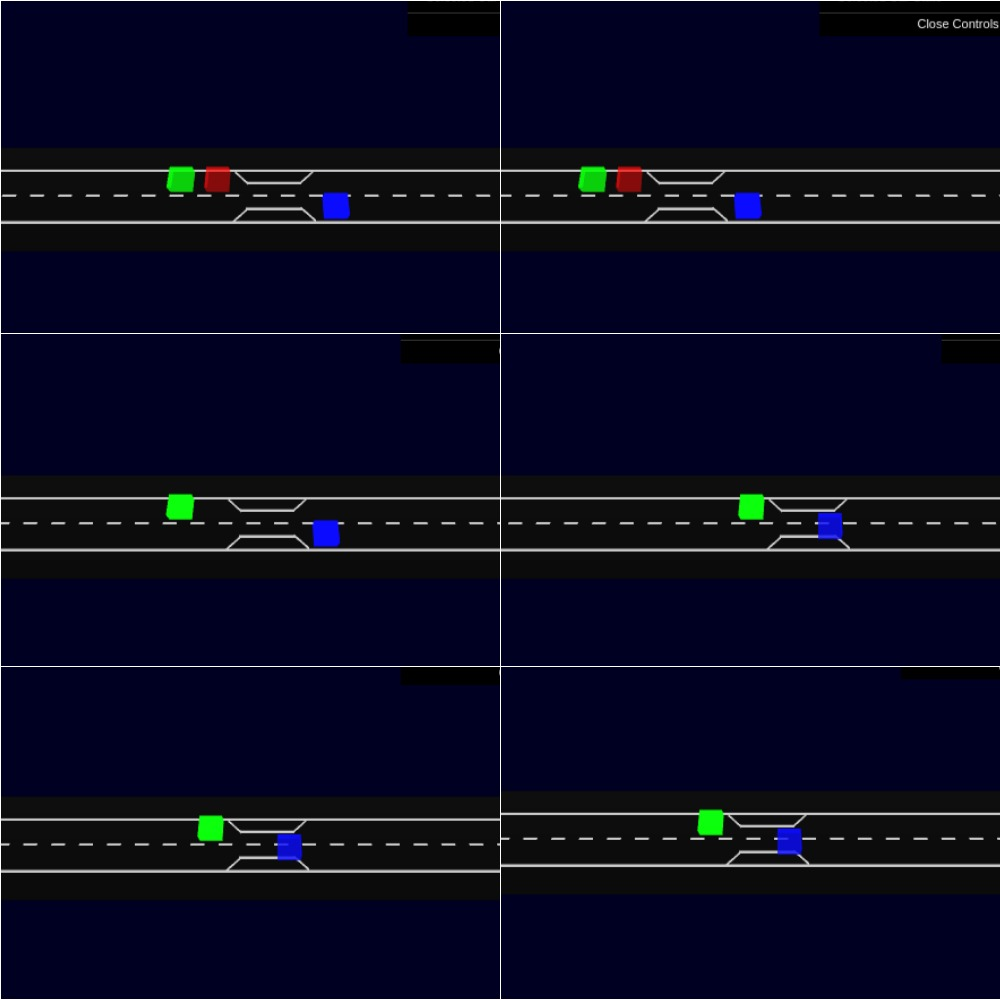
\includegraphics[scale=0.3, width=\linewidth]{assets/sc4.jpg}
        \captionof{figure}{scenery 4}
    \end{center}

    The correct behaviour should be that the two cars that won't have any type of crash
    will cross the bridge even if there is one in front of them that has crashed. Due to the fact that the 
    $crash\_type$ for the broken one is 2, the other cars (at least one of them) have to call the tow truck for 
    it; after it has been removed the cars can continue crossing the bridge \\

    \item[\fbox{scenery \textbf{5}} $\quad$] There are five cars that are on the same side and all of them have a crash; three of them have system crash, 
    while the other have only engine crash and there is a delay between the car with $crash\_type$ 2 and the others.\\
   
    \begin{center}
        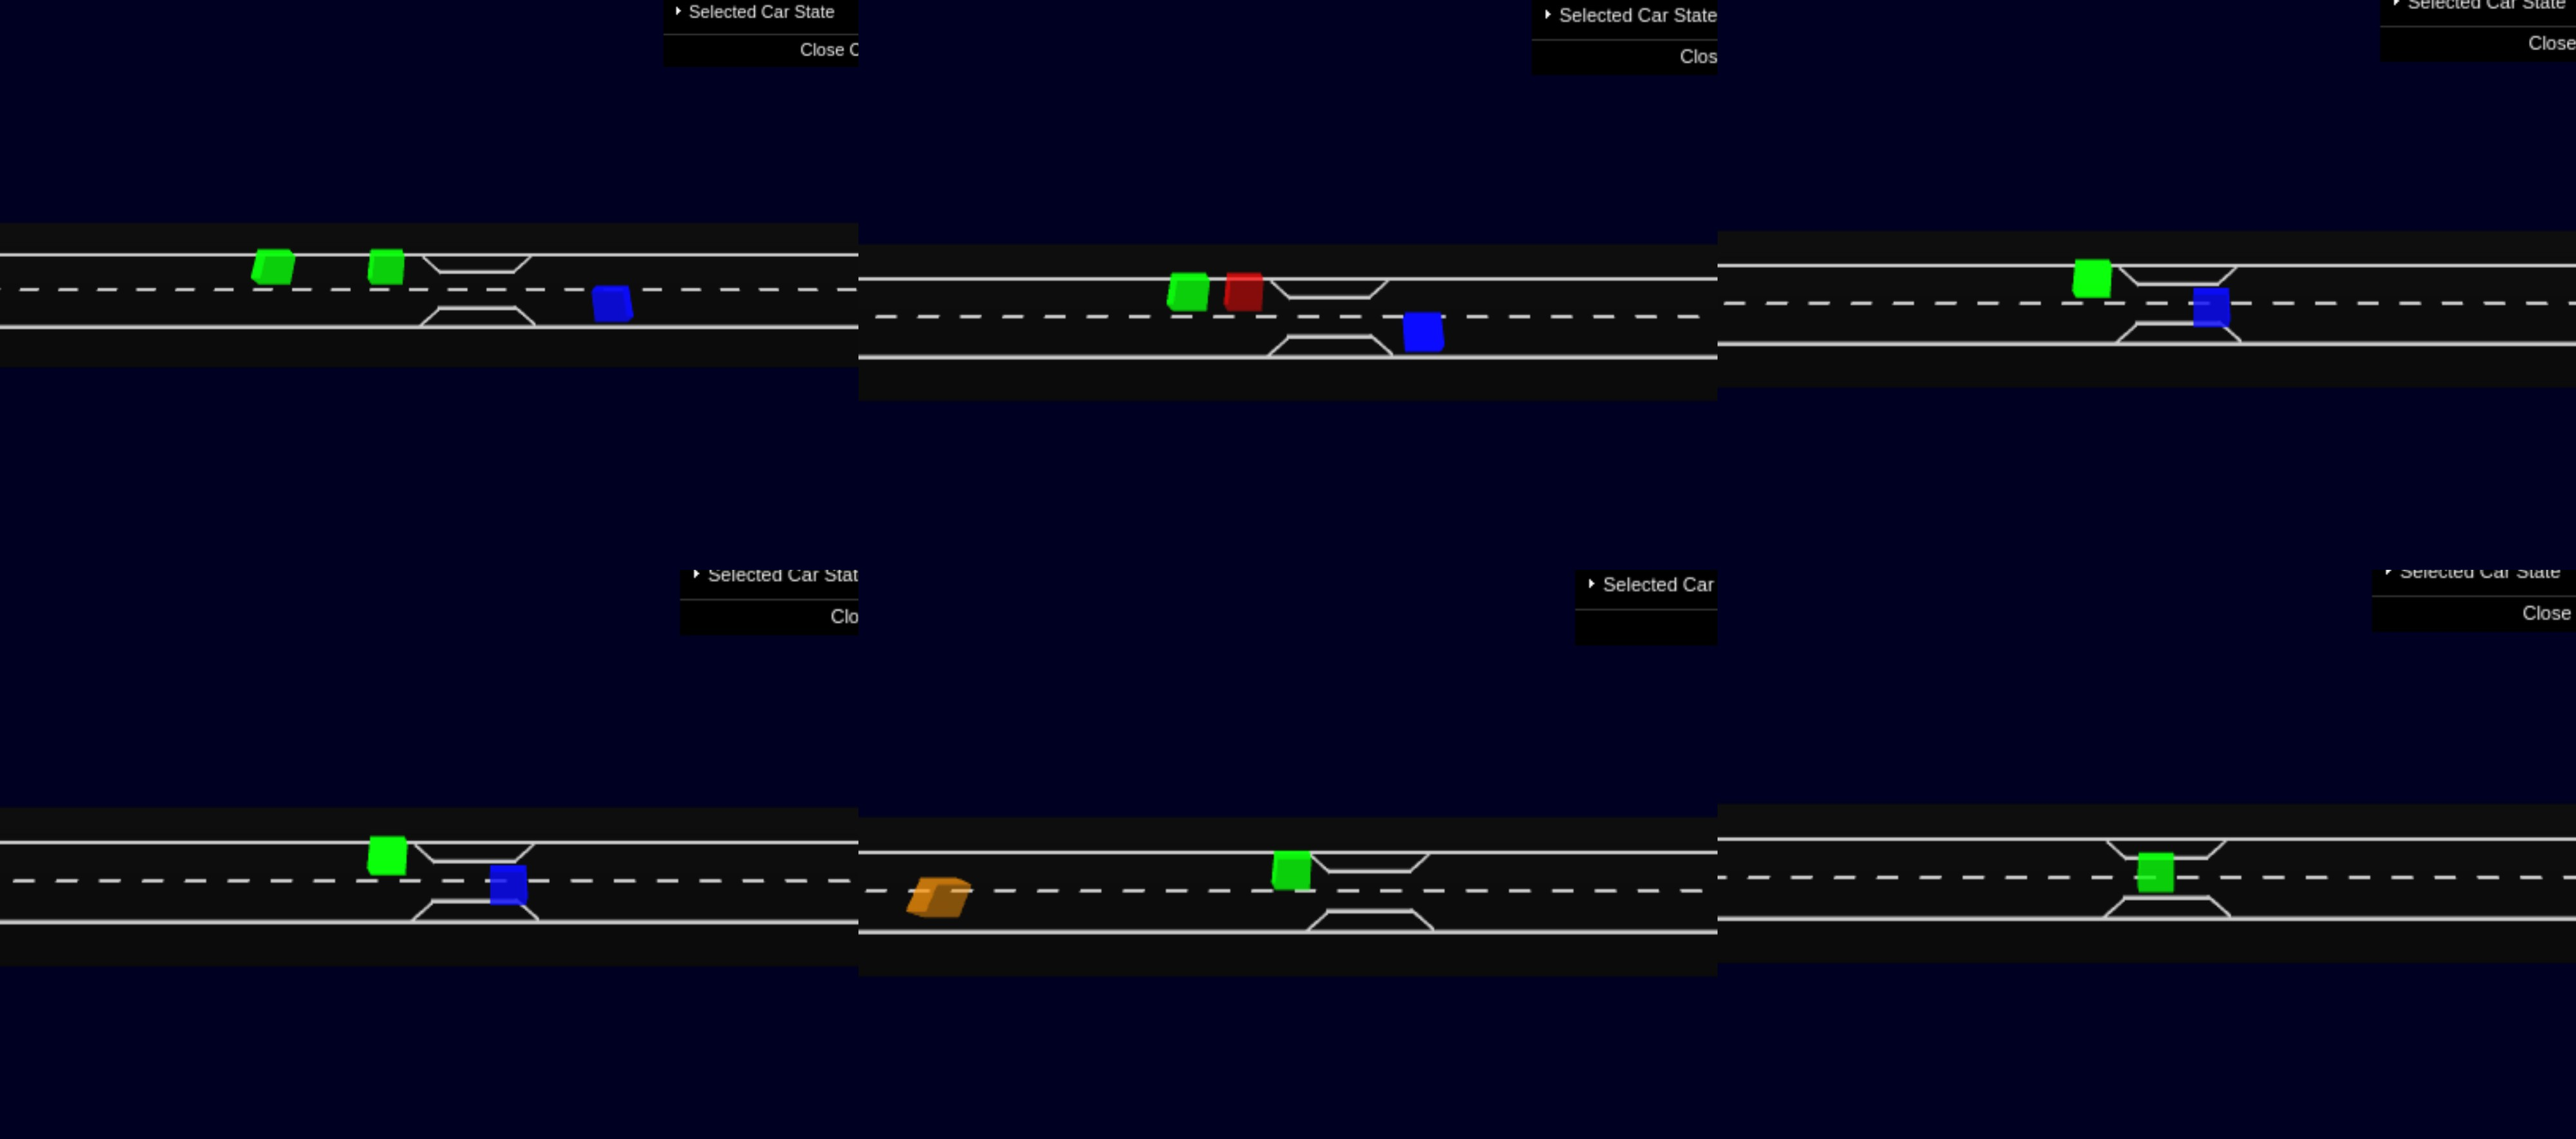
\includegraphics[scale=0.3, width=\linewidth]{assets/sc5.jpg}
        \captionof{figure}{scenery 5}
    \end{center}

    The correct behaviour should be that the cars that have only engine crash will call the tow truck for themselves and
    for the cars that they can reach (because if a car has system crash cannot call a tow truck for itself). 
    For this reason if there is a car that has a system crash after that the cars, which had an engine crash, 
    have already been removed by the tow truck, it will stuck there, waiting for a new car to call the tow truck for it\\

    \item[\fbox{scenery \textbf{6}} $\quad$] There are two cars that will have a crash with $crash\_type$ 2 and another one that will not
    crash and that will arrive after that the previously cars have crashed due to the delay between them. All of them are on the same 
    side of the bridge. \\ 
    \begin{center}
        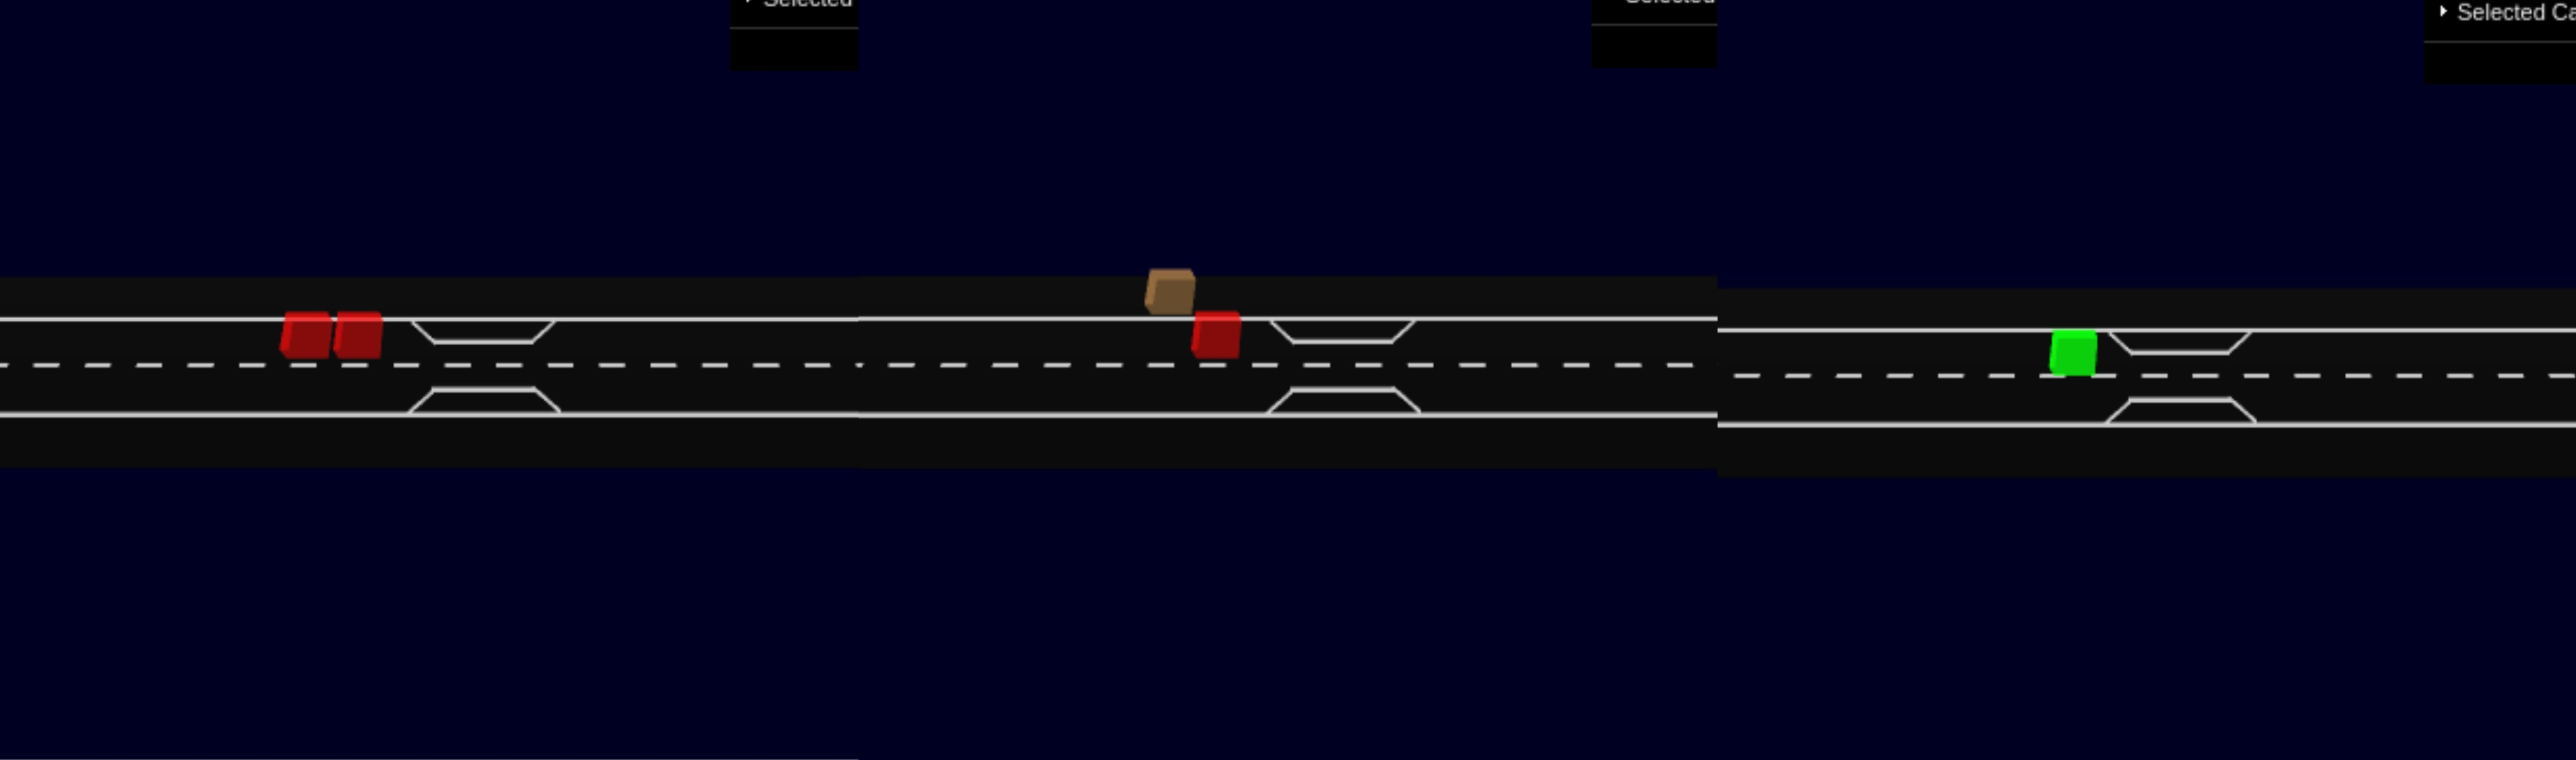
\includegraphics[scale=0.3, width=\linewidth]{assets/sc6.jpg}
        \captionof{figure}{scenery 6}
    \end{center}

    The correct behaviour should be that the cars with 
    the crash will wait there until the other one arrive and call a tow truck for them. After they have been removed
    the last car can cross the bridge \\

    \item[\fbox{scenery \textbf{7}} $\quad$] It is the same as the above but there are only two cars and them are on different sides; the 
    sane one has a delay. 

    \begin{center}
        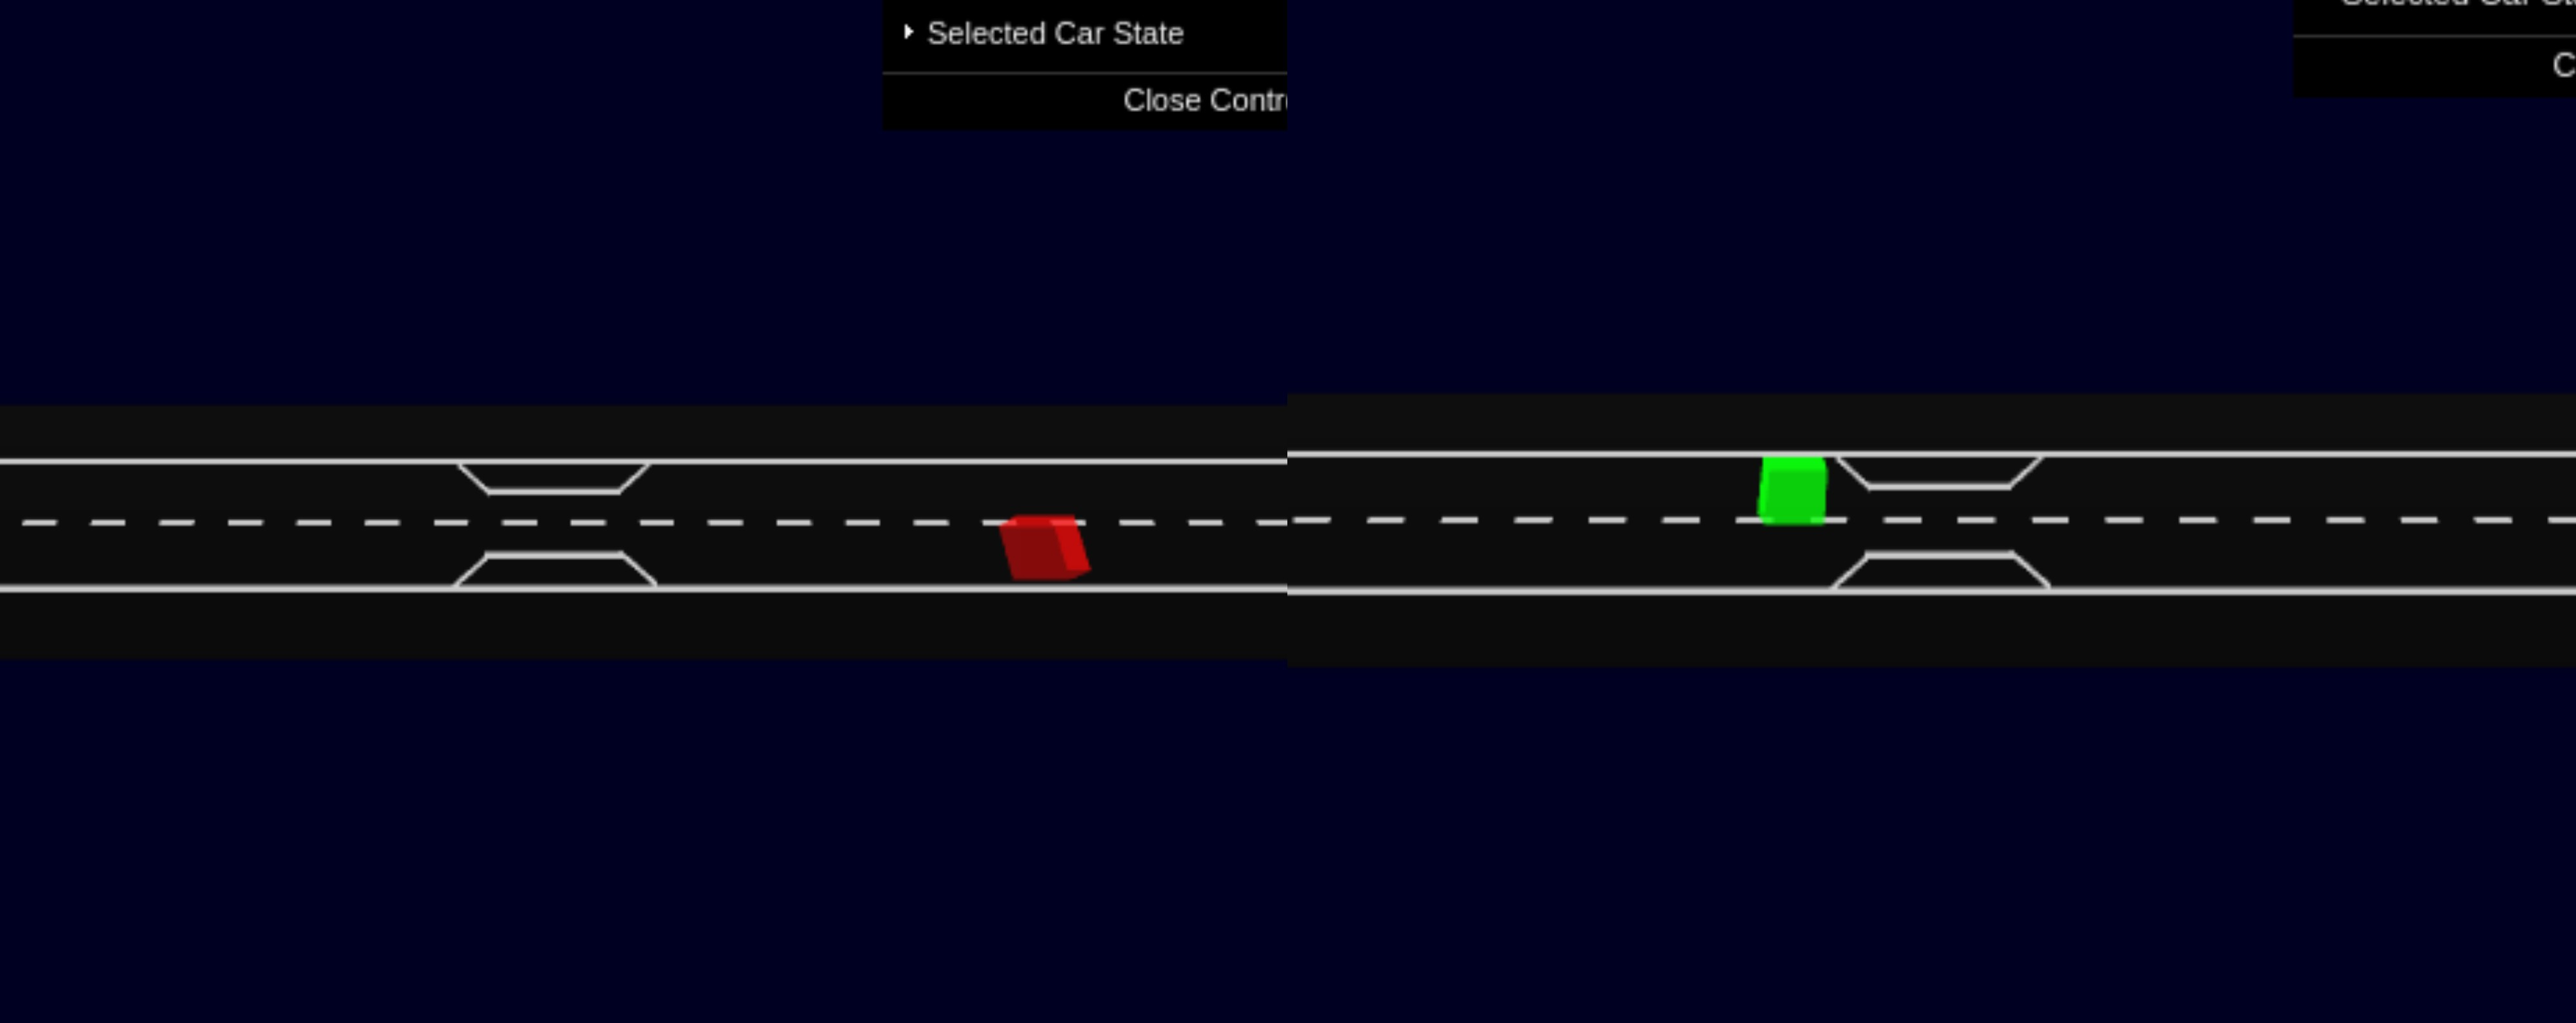
\includegraphics[scale=0.3, width=\linewidth]{assets/sc7.jpg}
        \captionof{figure}{scenery 7}
    \end{center}

    The correct behaviour should be that when it arrives, it will call the tow truck for
    the other and then cross the bridge (after the other has been removed) \\

   \item[\fbox{scenery \textbf{8}} $\quad$] There are five cars on the same side but only one (with the longer delay) is sane. \\
  
   \begin{center}
        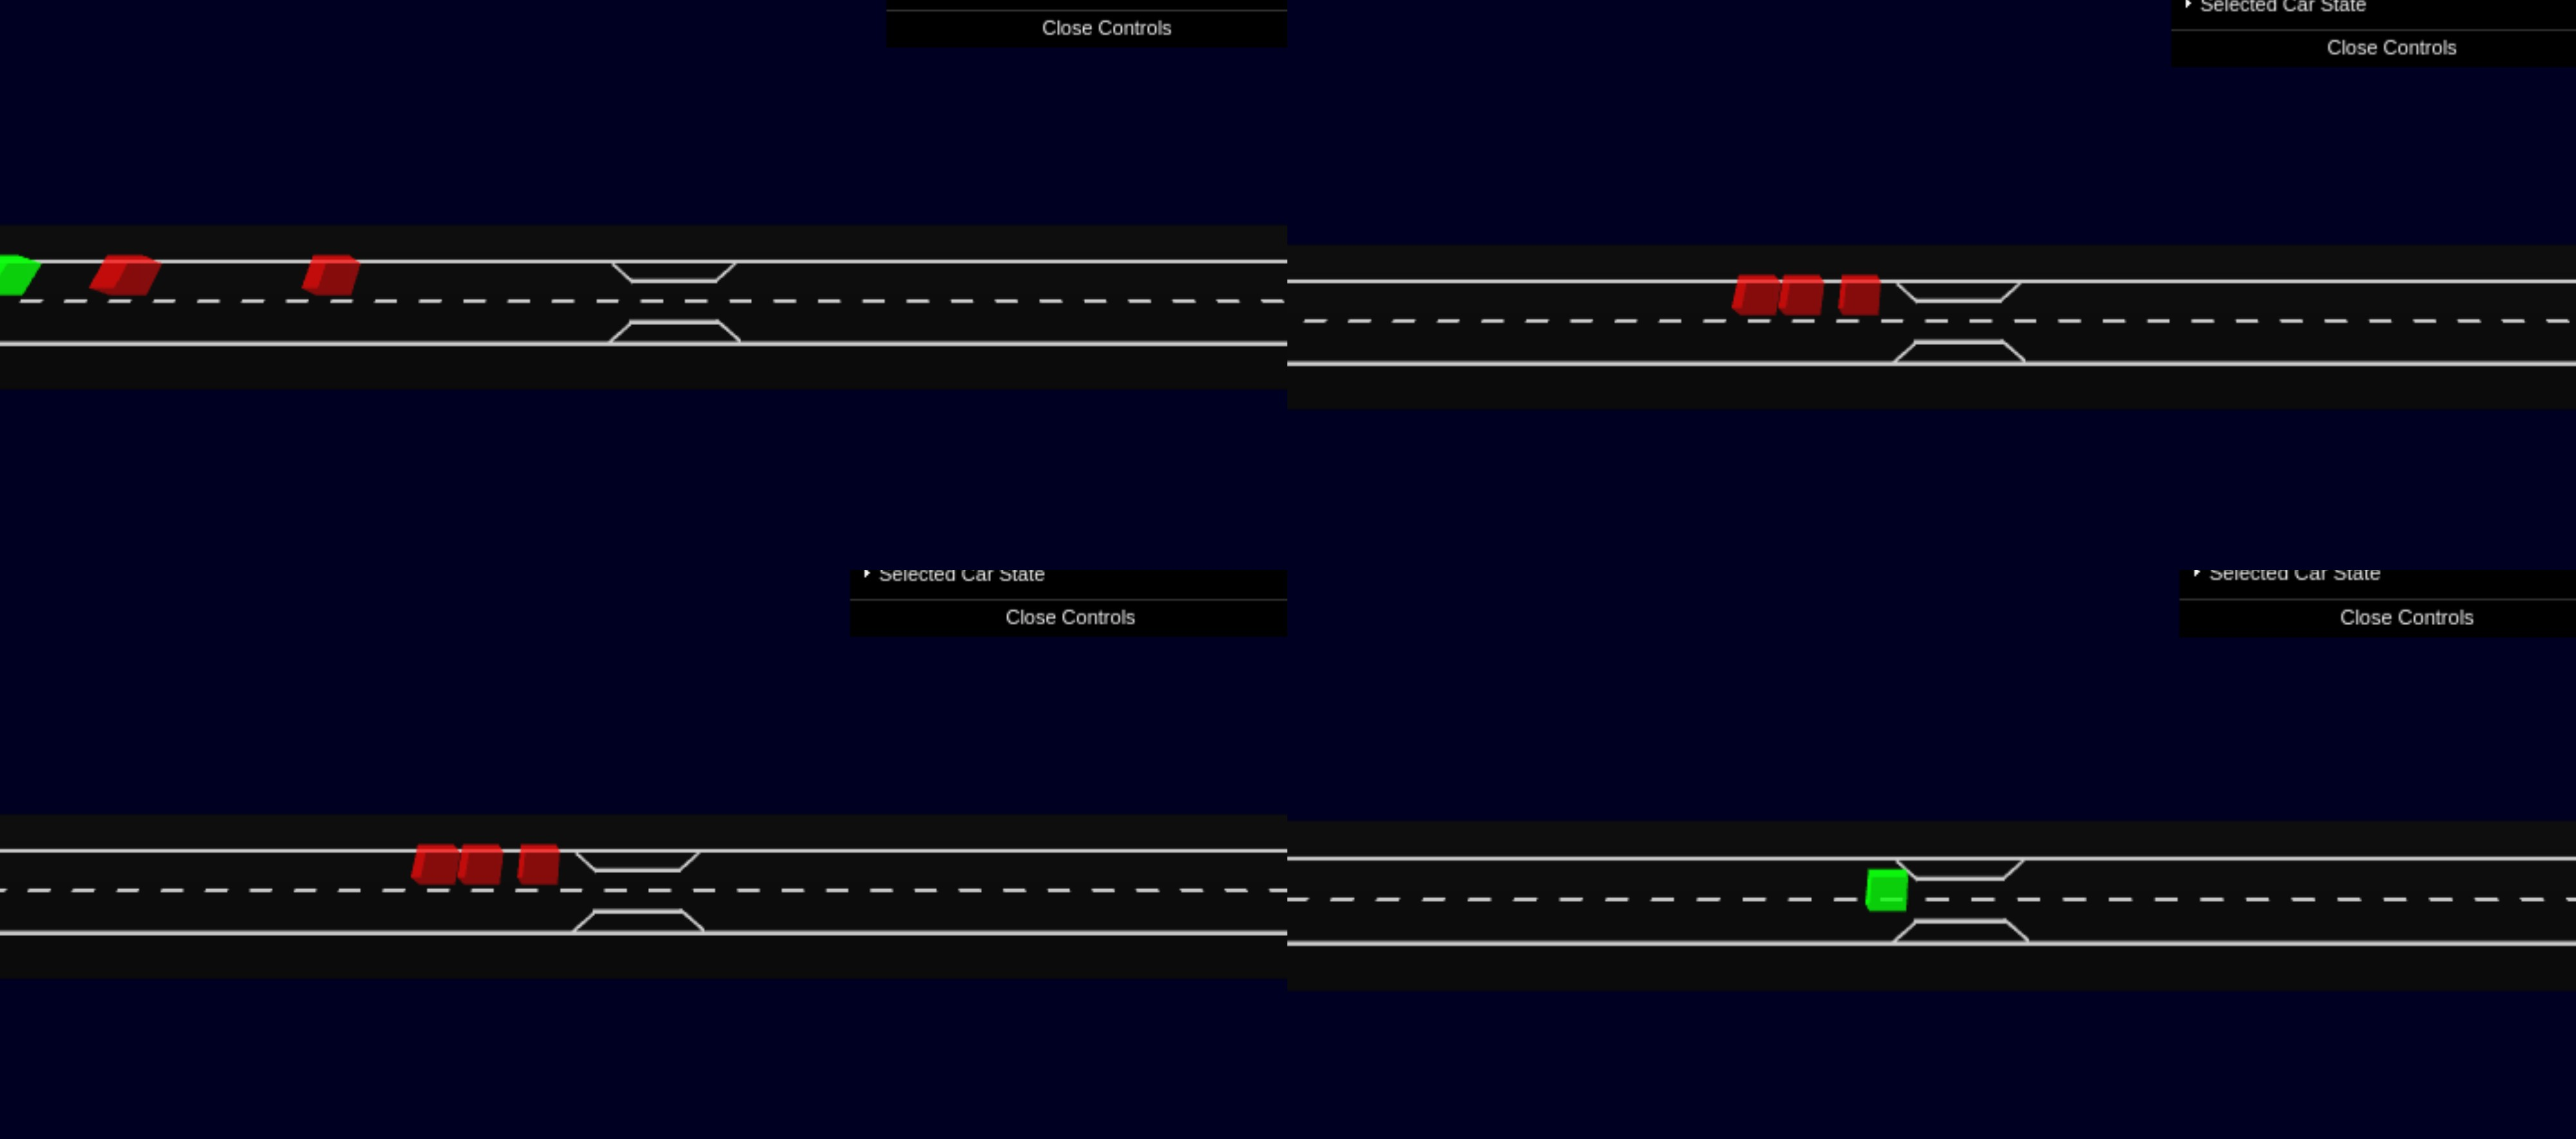
\includegraphics[scale=0.3, width=\linewidth]{assets/sc8.jpg}
        \captionof{figure}{scenery 8}
    \end{center} 

    The correct behaviour should be that the cars with crashes will wait to be removed by the tow truck called 
    by the sane one (they have $crash\_type$ 2) and then the last car can cross the bridge \\

    \item[\fbox{scenery \textbf{9}} $\quad$] There are three cars, two from the same side. One of them has a system crash 
    and a delay of 300ms. \\

    \begin{center}
        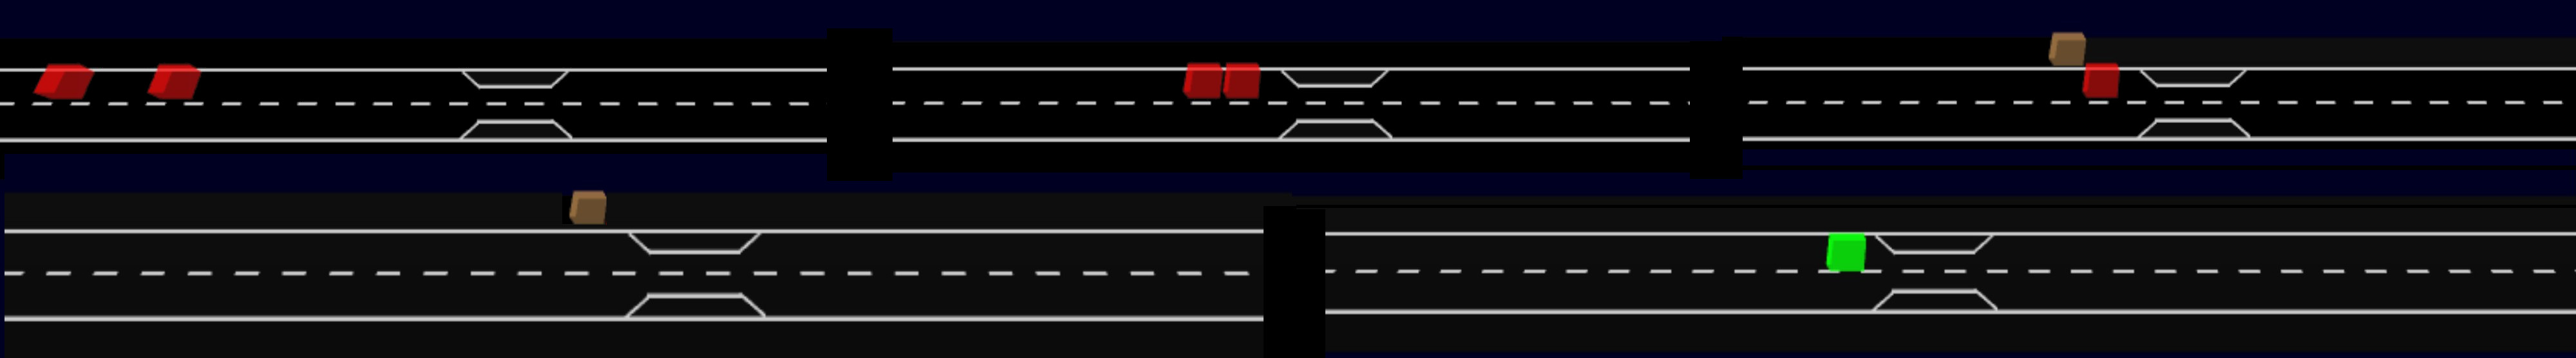
\includegraphics[scale=0.3, width=\linewidth]{assets/sc10.jpg}
        \captionof{figure}{scenery 9}
    \end{center}

    The correct behaviour should be that the car with crash will wait to be removed by the tow truck called by
    one or both the others cars.\\
\end{itemize}

We tested also others scenarys:
\begin{itemize}
    \item 9 other scenarys that are the same as the 9 already shown but with opposite side for each car (i.e. 
    if a scenary previously listed has two car, one from right and one from left, in the new scenary the right one
    would be on the left and the left one on the right)
    \item 6 other scenarys that are the same as the 6 already shown (but only these with cars that will crash) 
    but, in the new scenery, every car that has a $crash\_type$ 2 will have $crash\_type$ 1 and vice versa. This case
    is even symplier because the $crash\_type$ 1 allows the crashed car to call the tow truck by itself.
\end{itemize}
